\PassOptionsToPackage{unicode=true}{hyperref} % options for packages loaded elsewhere
\PassOptionsToPackage{hyphens}{url}
%
\documentclass[]{article}
\usepackage{lmodern}
\usepackage{amssymb,amsmath}
\usepackage{ifxetex,ifluatex}
\usepackage{fixltx2e} % provides \textsubscript
\ifnum 0\ifxetex 1\fi\ifluatex 1\fi=0 % if pdftex
  \usepackage[T1]{fontenc}
  \usepackage[utf8]{inputenc}
  \usepackage{textcomp} % provides euro and other symbols
\else % if luatex or xelatex
  \usepackage{unicode-math}
  \defaultfontfeatures{Ligatures=TeX,Scale=MatchLowercase}
\fi
% use upquote if available, for straight quotes in verbatim environments
\IfFileExists{upquote.sty}{\usepackage{upquote}}{}
% use microtype if available
\IfFileExists{microtype.sty}{%
\usepackage[]{microtype}
\UseMicrotypeSet[protrusion]{basicmath} % disable protrusion for tt fonts
}{}
\usepackage{hyperref}
\hypersetup{
            pdftitle={Concrete compressive strength prediction with machine learning},
            pdfauthor={Pedro Bernardino Alves Moreira},
            pdfborder={0 0 0},
            breaklinks=true}
\urlstyle{same}  % don't use monospace font for urls
\usepackage[margin=1in]{geometry}
\usepackage{graphicx,grffile}
\makeatletter
\def\maxwidth{\ifdim\Gin@nat@width>\linewidth\linewidth\else\Gin@nat@width\fi}
\def\maxheight{\ifdim\Gin@nat@height>\textheight\textheight\else\Gin@nat@height\fi}
\makeatother
% Scale images if necessary, so that they will not overflow the page
% margins by default, and it is still possible to overwrite the defaults
% using explicit options in \includegraphics[width, height, ...]{}
\setkeys{Gin}{width=\maxwidth,height=\maxheight,keepaspectratio}
\setlength{\emergencystretch}{3em}  % prevent overfull lines
\providecommand{\tightlist}{%
  \setlength{\itemsep}{0pt}\setlength{\parskip}{0pt}}
\setcounter{secnumdepth}{5}
% Redefines (sub)paragraphs to behave more like sections
\ifx\paragraph\undefined\else
\let\oldparagraph\paragraph
\renewcommand{\paragraph}[1]{\oldparagraph{#1}\mbox{}}
\fi
\ifx\subparagraph\undefined\else
\let\oldsubparagraph\subparagraph
\renewcommand{\subparagraph}[1]{\oldsubparagraph{#1}\mbox{}}
\fi

% set default figure placement to htbp
\makeatletter
\def\fps@figure{htbp}
\makeatother

\usepackage{booktabs}
\usepackage{longtable}
\usepackage{supertabular}
\usepackage{array}
\usepackage{multirow}
\usepackage{wrapfig}
\usepackage{colortbl}
\usepackage{pdflscape}
\usepackage{tabu}
\usepackage{threeparttable}
\usepackage[normalem]{ulem}
\usepackage{caption}
\usepackage{floatrow}
\floatsetup[table]{capposition=top}
\floatsetup[figure]{capposition=top}
\captionsetup{options=chunk}
\DeclareNewFloatType{chunk}{placement=H, fileext=chk, name=}
\renewcommand{\thechunk}{\arabic{chunk}}
\usepackage{indentfirst}
\usepackage{sectsty} \sectionfont{\centering}
\usepackage{booktabs}
\usepackage{longtable}
\usepackage{array}
\usepackage{multirow}
\usepackage{wrapfig}
\usepackage{float}
\usepackage{colortbl}
\usepackage{pdflscape}
\usepackage{tabu}
\usepackage{threeparttable}
\usepackage{threeparttablex}
\usepackage[normalem]{ulem}
\usepackage{makecell}
\usepackage{xcolor}

\title{Concrete compressive strength prediction with machine learning}
\author{Pedro Bernardino Alves Moreira}
\date{April 22, 2020}

\begin{document}
\maketitle
\begin{abstract}
Compressive strength is the main characteristic of concrete. The correct
prediction of this parameter means cost and time reduction. This work
built predictive models for 6 different ages of concrete samples (3, 7,
14, 28, 56, and 100 days). A set of data obtained in previous studies
was used, a total of 1030 samples, with 9 variables: compressive
strength, age, and 7 ingredients (water, cement, fine aggregate, coarse
aggregate, fly ash, blast furnace slag, and superplasticizers). Another
6 variables were added to represent the proportions of the main
ingredients in each sample (water/cement, fine aggregate/cement, coarse
aggregate/cement, fine aggregate/coarse aggregate, water/coarse
aggregate, and water/fine aggregate). The predictive models were
developed in \emph{R} language, using the \emph{caret} package with the
\emph{Parallel Random Forest} algorithm and repeated cross-validation
technique to optimize the parameters. The results were satisfactory and
compatible with other studies using the same data set. The most
important model, 28 days old, obtained \emph{RMSE} of 4.717. The 3-day
model obtained the best result, \emph{RMSE} of 3.310. The worst result
was the 56-day model, with \emph{RMSE} of 5.939. The work showed that
the compressive strength of concrete can be predicted. The choice of
creating a model for each age, instead of using age as a predictor,
allowed to get compatible results with the available data at each age.
It was a promising alternative since good results were achieved by
training with just one algorithm. This work facilitates exploration and
new efforts to predict the compressive strength of concrete, it can be
replicated using different algorithms or the combination of several.
\end{abstract}

\newpage
\tableofcontents
\newpage
\listoffigures
\listoftables
\newpage

\hypertarget{introduction}{%
\section{Introduction}\label{introduction}}

Compressive strength is the main characteristic of concrete, measured by
tests of international standards that consist of the breaking of
specimens. Measurement at 28 days is mandatory and represents the grade
of the concrete. Knowing in advance what the result will be obtained for
a given age, based on the proportions of its ingredients, is of great
interest to concrete manufacturers, construction companies, and civil
engineers.

~

This compressive strength is a nonlinear function of its ingredients and
age, making it difficult to establish an analytical formula, although
some formulas have already been proposed. ({\textbf{???}}) proposed a
mathematical model to predict from the results of tests of 7 and 14
days, and ({\textbf{???}}) from 7 days. However, machine learning
techniques can be used to model this characteristic from real sample
data, using only the ingredients.

~

Many previous studies use the same dataset used by Yeh (n.d.) to predict
the compressive strength of concrete. ({\textbf{???}}) got good results
with the regularized extreme learning machine (RELM) technique, and
({\textbf{???}}) got even better results with the Artificial Neural
Networks and cross-validation technique. This set of samples is so well
known that there are many pages on the internet of unpublished studies
that use it and have good results, such as ({\textbf{???}}),
({\textbf{???}}), ({\textbf{???}}) and ({\textbf{???}}). At the end of
the work, the results found are compared to the works cited here.

~

Unlike previous studies with this dataset, this work does data
preparation differently. The age of the concrete is the most unique
feature that contributes to its compressive strength. For this reason,
age is treated separately in the machine learning models, creating
models for each age group.

\hypertarget{materials-and-methods}{%
\section{Materials and Methods}\label{materials-and-methods}}

\hypertarget{materials}{%
\subsection{Materials}\label{materials}}

The methodology was carried out using RStudio software ({\textbf{???}}),
an integrated virtual environment for code development in \emph{R}
({\textbf{???}}). Throughout the process, all code executed was
documented in the same order as its execution in
\protect\hyperlink{appendix2}{Appendix 2}, and reference was always made
to codes throughout the text. All relevant information related to the
operating system and installed packages has been presented in
\protect\hyperlink{appendix1}{Appendix 1}.

\hypertarget{reproducibility}{%
\subsection{Reproducibility}\label{reproducibility}}

In order to guarantee reproducibility, whenever there was some code that
could use probabilistic operations, a \emph{seed} was defined before its
execution, ensuring that when run on another machine, with the same
version of \emph{R} and the same \emph{seed}, get the same result. The
\emph{seeds} can be checked throughout
\protect\hyperlink{appendix2}{Appendix 2}.

\hypertarget{obtaining-the-data}{%
\subsection{Obtaining the data}\label{obtaining-the-data}}

The data was downloaded from the University of California Irvine website
({\textbf{???}}) (\ref{show-download-data}). In total there are 1030
samples with 9 columns. The samples were renamed and an id column was
added to facilitate data manipulation (\ref{show-rename-dat-cols}). The
columns were reordered to put the new id column in the first position
(\ref{show-reorder-dat}). The first samples can be viewed in the table
\ref{tab:first-samples}.

~

\begin{table}[H]

\caption{\label{tab:first-samples}First 6 samples}
\centering
\resizebox{\linewidth}{!}{
\begin{tabular}[t]{cccccccccc}
\toprule
\multicolumn{1}{c}{ID} & \multicolumn{1}{c}{Cement} & \multicolumn{1}{c}{B.F.S.} & \multicolumn{1}{c}{Fly ash} & \multicolumn{1}{c}{Water} & \multicolumn{1}{c}{Superp.} & \multicolumn{1}{c}{C.Aggregate} & \multicolumn{1}{c}{F.Aggregate} & \multicolumn{1}{c}{Day} & \multicolumn{1}{c}{Comp.Str.} \\
 & $kg/m^3$ & $kg/m^3$ & $kg/m^3$ & $kg/m^3$ & $kg/m^3$ & $kg/m^3$ & $kg/m^3$ &  & $MPa$\\
\midrule
1 & 540.0 & 0.0 & 0 & 162 & 2.5 & 1040.0 & 676.0 & 28 & 79.99\\
\addlinespace
2 & 540.0 & 0.0 & 0 & 162 & 2.5 & 1055.0 & 676.0 & 28 & 61.89\\
\addlinespace
3 & 332.5 & 142.5 & 0 & 228 & 0.0 & 932.0 & 594.0 & 270 & 40.27\\
\addlinespace
4 & 332.5 & 142.5 & 0 & 228 & 0.0 & 932.0 & 594.0 & 365 & 41.05\\
\addlinespace
5 & 198.6 & 132.4 & 0 & 192 & 0.0 & 978.4 & 825.5 & 360 & 44.30\\
\addlinespace
6 & 266.0 & 114.0 & 0 & 228 & 0.0 & 932.0 & 670.0 & 90 & 47.03\\
\bottomrule
\end{tabular}}
\end{table}

\hypertarget{data-preparation}{%
\subsection{Data preparation}\label{data-preparation}}

The preparation of the data consisted of transforming the sample set in
order to maintain only relevant data for the subsequent studies. Data
that were considered irrelevant or that had the potential to add
undesirable noise to the analysis were removed. In addition, the
relevant data has been transformed to better fit the studies in the next
steps.

\hypertarget{initial-data-cleaning}{%
\subsubsection{Initial data cleaning}\label{initial-data-cleaning}}

Initially, there were 25 duplicate samples that were removed, resulting
in a new total of 1005 samples (\ref{show-removing-duplicated-samples}).

~

The data show the variables in the columns and samples in the rows.
However it was found that some samples are identical in proportions of
ingredients, changing only the value of age and compressive strength,
for example, samples 653, 654, 678 and 681, shown in the table
\ref{tab:similar-samples}.

~

\begin{table}[H]

\caption{\label{tab:similar-samples}Samples with same composition}
\centering
\resizebox{\linewidth}{!}{
\begin{tabular}[t]{cccccccccc}
\toprule
\multicolumn{1}{c}{ID} & \multicolumn{1}{c}{Cement} & \multicolumn{1}{c}{B.F.S.} & \multicolumn{1}{c}{Fly ash} & \multicolumn{1}{c}{Water} & \multicolumn{1}{c}{Superp.} & \multicolumn{1}{c}{C.Aggregate} & \multicolumn{1}{c}{F.Aggregate} & \multicolumn{1}{c}{Day} & \multicolumn{1}{c}{Comp.Str.} \\
 & $kg/m^3$ & $kg/m^3$ & $kg/m^3$ & $kg/m^3$ & $kg/m^3$ & $kg/m^3$ & $kg/m^3$ &  & $MPa$\\
\midrule
653 & 102 & 153 & 0 & 192 & 0 & 887 & 942 & 3 & 4.57\\
\addlinespace
678 & 102 & 153 & 0 & 192 & 0 & 887 & 942 & 7 & 7.68\\
\addlinespace
681 & 102 & 153 & 0 & 192 & 0 & 887 & 942 & 28 & 17.28\\
\addlinespace
654 & 102 & 153 & 0 & 192 & 0 & 887 & 942 & 90 & 25.46\\
\bottomrule
\end{tabular}}
\end{table}

In addition, there are also samples with the same values and proportions
of ingredients, but with different compressive strength, probably due to
differences in the building process. This is the case, for example, of
samples 472, 473 and 474, shown in the table
\ref{tab:similar-samples-2}.

~

\begin{table}

\caption{\label{tab:similar-samples-2}Same samples with different results}
\centering
\resizebox{\linewidth}{!}{
\begin{tabular}[t]{cccccccccc}
\toprule
\multicolumn{1}{c}{ID} & \multicolumn{1}{c}{Cement} & \multicolumn{1}{c}{B.F.S.} & \multicolumn{1}{c}{Fly ash} & \multicolumn{1}{c}{Water} & \multicolumn{1}{c}{Superp.} & \multicolumn{1}{c}{C.Aggregate} & \multicolumn{1}{c}{F.Aggregate} & \multicolumn{1}{c}{Day} & \multicolumn{1}{c}{Comp.Str.} \\
 & $kg/m^3$ & $kg/m^3$ & $kg/m^3$ & $kg/m^3$ & $kg/m^3$ & $kg/m^3$ & $kg/m^3$ &  & $MPa$\\
\midrule
472 & 446 & 24 & 79 & 162 & 11.6 & 967 & 712 & 28 & 57.03\\
\addlinespace
473 & 446 & 24 & 79 & 162 & 11.6 & 967 & 712 & 28 & 44.42\\
\addlinespace
474 & 446 & 24 & 79 & 162 & 11.6 & 967 & 712 & 28 & 51.02\\
\bottomrule
\end{tabular}}
\end{table}

To facilitate the analysis of the samples, all samples that are the same
in relation to the ingredients, have been assigned the same \emph{id}.
In addition, as the compressive strength at 28 days is the parameter to
determine the grade of the concrete, only the elements containing that
day among its samples were maintained. In the case of the same samples
but with different results of compressive strength, the values were
averaged. After all these changes (\ref{show-initial-data-cleaning}),
the new total of samples was reduced to 970, containing 416 different
settings for the proportions of ingredients.

~

The result can be seen in the table \ref{tab:similar-samples-same-id}.
All samples with equal ingredient settings have the same id, and when
they had different results for the same days, they were transformed into
just one sample, with the arithmetic mean in the compressive strength.

~

\begin{table}[H]

\caption{\label{tab:similar-samples-same-id}Previous samples after processing}
\centering
\resizebox{\linewidth}{!}{
\begin{tabular}[t]{cccccccccc}
\toprule
\multicolumn{1}{c}{ID} & \multicolumn{1}{c}{Cement} & \multicolumn{1}{c}{B.F.S.} & \multicolumn{1}{c}{Fly ash} & \multicolumn{1}{c}{Water} & \multicolumn{1}{c}{Superp.} & \multicolumn{1}{c}{C.Aggregate} & \multicolumn{1}{c}{F.Aggregate} & \multicolumn{1}{c}{Day} & \multicolumn{1}{c}{Comp.Str.} \\
 & $kg/m^3$ & $kg/m^3$ & $kg/m^3$ & $kg/m^3$ & $kg/m^3$ & $kg/m^3$ & $kg/m^3$ &  & $MPa$\\
\midrule
472 & 446 & 24 & 79 & 162 & 11.6 & 967 & 712 & 28 & 50.82\\
\addlinespace
653 & 102 & 153 & 0 & 192 & 0.0 & 887 & 942 & 3 & 4.57\\
\addlinespace
653 & 102 & 153 & 0 & 192 & 0.0 & 887 & 942 & 7 & 7.68\\
\addlinespace
653 & 102 & 153 & 0 & 192 & 0.0 & 887 & 942 & 28 & 17.28\\
\addlinespace
653 & 102 & 153 & 0 & 192 & 0.0 & 887 & 942 & 90 & 25.46\\
\bottomrule
\end{tabular}}
\end{table}

\hypertarget{age-selection}{%
\subsubsection{Age selection}\label{age-selection}}

As previously described, the main age for analysis of compressive
strength is 28 days, but other ages can also be used to build predictive
models. However, it is necessary to verify how relevant the data of
these other ages are. Starting with the distribution of the samples in
relation to each age (\ref{show-boxplot}) shown in the figure
\ref{fig:boxplot}.

~

\begin{figure}

{\centering 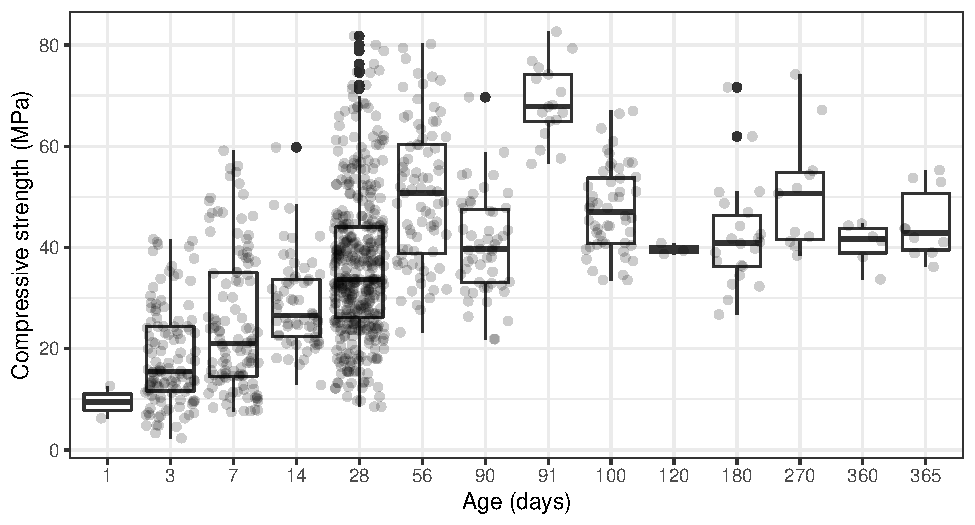
\includegraphics{CopyOfcapstone_files/figure-latex/boxplot-1} 

}

\caption{Boxplot - Compressive strength (MPa) vs age (days)}\label{fig:boxplot}
\end{figure}

It was observed that the ages of 90, 91 and 100 days probably represent
extremes to each other in the ingredient configurations, since they are
relatively close ages but with very different values, especially for 90
and 91.

~

This hypothesis was verified using the principal component analysis
method, applied to samples of these 3 ages (\ref{show-pca-90-91-100}).
The figure \ref{fig:pca-90-91-100} shows how the samples relate to each
other (which are similar or different) and revealed how each variable
contributes to the analysis. The first two dimensions represent 37\% and
24\% \$ respectively of the variance.

~

\begin{figure}

{\centering 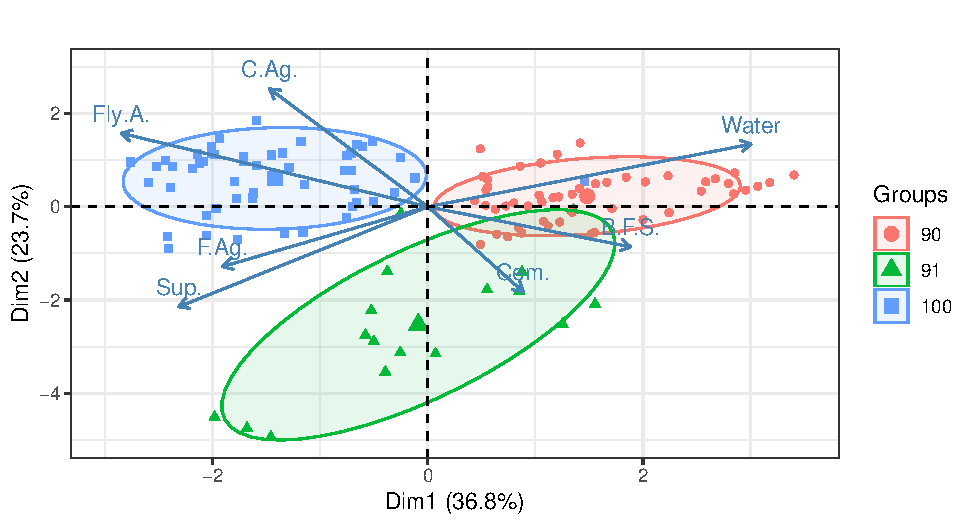
\includegraphics{CopyOfcapstone_files/figure-latex/pca-90-91-100-1} 

}

\caption{Principal component analysis - 90, 91 e 100 days}\label{fig:pca-90-91-100}
\end{figure}

Another important point considered, of the concrete nature itself, is
the fact that the growth rate of its compressive strength decreases with
time, reaching a certain stability value. The figure
\ref{fig:mpa-on-time} shows the compressive strength over the days for
samples with more than 5 data, that is, data available for at least 6
different ages (\ref{show-mpa-on-time}).

~

\begin{figure}

{\centering 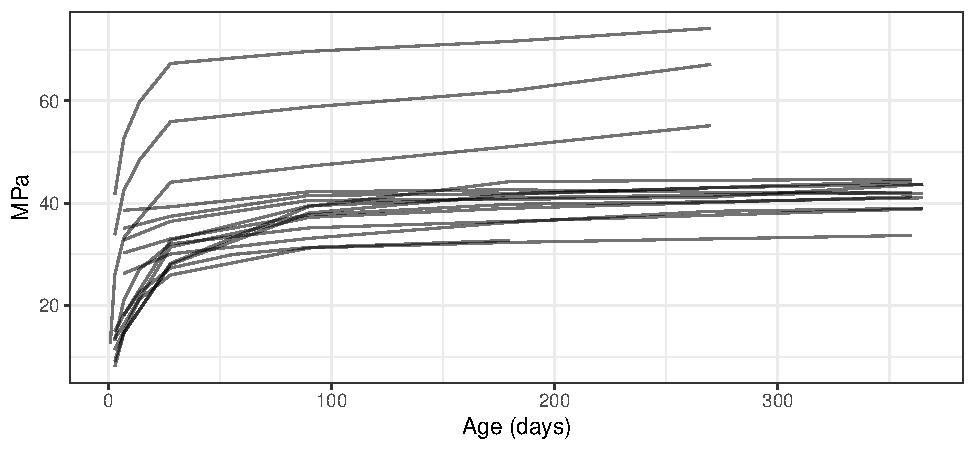
\includegraphics{CopyOfcapstone_files/figure-latex/mpa-on-time-1} 

}

\caption{Compressive strength through time}\label{fig:mpa-on-time}
\end{figure}

For the reasons presented in the figures \ref{fig:boxplot},
\ref{fig:pca-90-91-100} and \ref{fig:mpa-on-time}, it was considered
that the ages of 90, 91 and 100 days can be grouped to improve reading
and decrease sample noise. They were converted to the same value, the
age of 100 days was chosen (\ref{show-join-90-91-100}). As shown in the
figure \ref{fig:mpa-on-time}, the resistance only increases, after 100
days the resistance to compression will be greater than or equal to the
value of 90 or 91 days.

~

Another topic analyzed in the selection of ages was the observed
frequency of each age value after this transformation from 90, 91 in 100
days, shown in the figure \ref{fig:freq-ages}. Some values of days have
very low concentrations of samples, at the risk of damaging more than
helping to create the models, so they were removed
(\ref{show-remove-ages-lower-50}). The criterion adopted was to maintain
only ages with a frequency greater than 50, only the values of 3, 7, 14,
28, 56 and 100 days.

~

\begin{figure}

{\centering 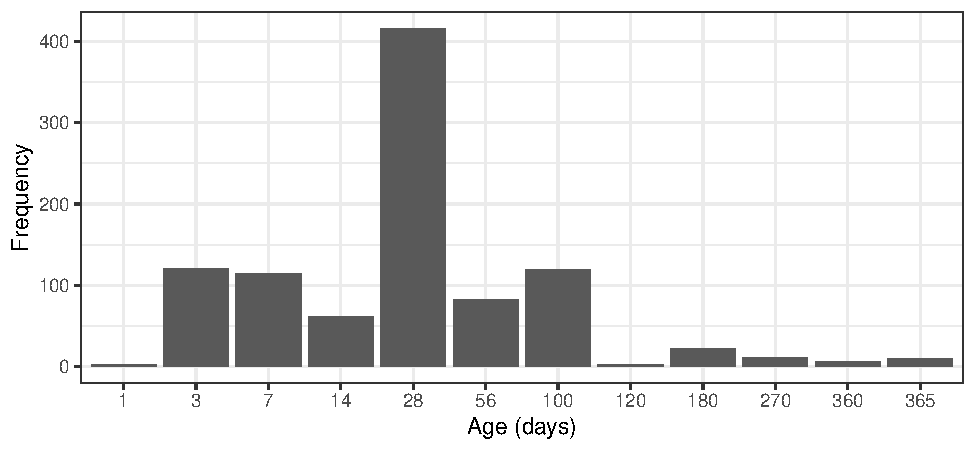
\includegraphics{CopyOfcapstone_files/figure-latex/freq-ages-1} 

}

\caption{Ages frequency}\label{fig:freq-ages}
\end{figure}

\hypertarget{data-reorganization}{%
\subsubsection{Data reorganization}\label{data-reorganization}}

The samples were grouped to maintain only one sample from each set of
configuration of the proportions of the ingredients, adding new
variables/columns for resistance at each age
(\ref{show-reorganizing-dat}). The result in the first samples after
this processing is shown in the table \ref{tab:new-features}.

~

\begin{table}[H]

\caption{\label{tab:new-features}First 6 samples after reorganization}
\centering
\resizebox{\linewidth}{!}{
\begin{tabular}[t]{cccccccccccccc}
\toprule
\multicolumn{1}{c}{ID} & \multicolumn{1}{c}{Cement} & \multicolumn{1}{c}{B.F.S} & \multicolumn{1}{c}{Fly ash} & \multicolumn{1}{c}{Water} & \multicolumn{1}{c}{Superp.} & \multicolumn{1}{c}{Coarse Ag.} & \multicolumn{1}{c}{Fine Ag.} & \multicolumn{1}{c}{3 days} & \multicolumn{1}{c}{7 days} & \multicolumn{1}{c}{14 days} & \multicolumn{1}{c}{28 days} & \multicolumn{1}{c}{56 days} & \multicolumn{1}{c}{100 days} \\
 & $kg/m^3$ & $kg/m^3$ & $kg/m^3$ & $kg/m^3$ & $kg/m^3$ & $kg/m^3$ & $kg/m^3$ & $MPa$ & $MPa$ & $MPa$ & $MPa$ & $MPa$ & $MPa$\\
\midrule
1 & 540.0 & 0.0 & 0 & 162 & 2.5 & 1040.0 & 676.0 &  &  &  & 79.99 &  & \\
\addlinespace
2 & 540.0 & 0.0 & 0 & 162 & 2.5 & 1055.0 & 676.0 &  &  &  & 61.89 &  & \\
\addlinespace
3 & 332.5 & 142.5 & 0 & 228 & 0.0 & 932.0 & 594.0 &  & 30.28 &  & 33.02 &  & 37.72\\
\addlinespace
5 & 198.6 & 132.4 & 0 & 192 & 0.0 & 978.4 & 825.5 & 9.13 & 14.64 &  & 28.02 &  & 38.07\\
\addlinespace
6 & 266.0 & 114.0 & 0 & 228 & 0.0 & 932.0 & 670.0 &  &  &  & 45.85 &  & 47.03\\
\addlinespace
7 & 380.0 & 95.0 & 0 & 228 & 0.0 & 932.0 & 594.0 &  & 32.82 &  & 36.45 &  & 40.56\\
\bottomrule
\end{tabular}}
\end{table}

The number of samples and distinct samples after all this manipulation
remained the same, a total of 416 (\ref{show-total-samples-2}).

\hypertarget{adding-new-variables}{%
\subsubsection{Adding new variables}\label{adding-new-variables}}

To finish the data preparation, new columns were added to the dataset
(\ref{show-new-features-2}). Starting with the concrete class, for
example if the compressive strength is between 25 and 30, it receives
the class \emph{C25}. The inclusion of the class was important because
the compressive strength in \emph{MPa} is a continuous variable, which
will be used in the regression models, but the class as a discrete
variable can provide another visualization of the data. The approximate
mix of concrete was also added, which represents the proportions of
aggregates (fine and coarse) for cement. Other proportions between the
main ingredients were also added. The new variables are presented in the
table \ref{tab:new-features-table}.

\begin{table}[H]

\caption{\label{tab:new-features-table}New features}
\centering
\resizebox{\linewidth}{!}{
\begin{tabular}[t]{c>{\centering\arraybackslash}p{1.5cm}>{\centering\arraybackslash}p{2cm}>{\centering\arraybackslash}p{1.7cm}>{\centering\arraybackslash}p{1.7cm}>{\centering\arraybackslash}p{1.7cm}>{\centering\arraybackslash}p{1.7cm}>{\centering\arraybackslash}p{1.7cm}>{\centering\arraybackslash}p{1.7cm}}
\toprule
ID & Class & Approximated Mix & Water / Cement & Fine Ag. / Cement & Coarse Ag. / Cement & Fine Ag. / Coarse Ag. & Water / Coarse Ag. & Water / Fine Ag.\\
\midrule
1 & C75 & 1:1:2 & 0.3000 & 1.2519 & 1.9259 & 0.6500 & 0.1558 & 0.2396\\
\addlinespace
2 & C60 & 1:1:2 & 0.3000 & 1.2519 & 1.9537 & 0.6408 & 0.1536 & 0.2396\\
\addlinespace
3 & C30 & 1:2:3 & 0.6857 & 1.7865 & 2.8030 & 0.6373 & 0.2446 & 0.3838\\
\addlinespace
5 & C25 & 1:4:5 & 0.9668 & 4.1566 & 4.9265 & 0.8437 & 0.1962 & 0.2326\\
\addlinespace
6 & C45 & 1:3:4 & 0.8571 & 2.5188 & 3.5038 & 0.7189 & 0.2446 & 0.3403\\
\addlinespace
7 & C35 & 1:2:2 & 0.6000 & 1.5632 & 2.4526 & 0.6373 & 0.2446 & 0.3838\\
\bottomrule
\end{tabular}}
\end{table}

\hypertarget{data-visualization}{%
\subsection{Data visualization}\label{data-visualization}}

In order to assess the need for further manipulation before building the
models, in this step the 416 samples already processed were visualized
and analyzed.

\hypertarget{descriptive-statistics}{%
\subsubsection{Descriptive statistics}\label{descriptive-statistics}}

The table \ref{tab:stat-summ} presents the statistical data of the
continuous variables (\ref {show-stat-summ}). The \emph{Null} line
represents the number of zeroed values for the ingredients, and the
\emph{NA} line represents the number of missing data. As the samples
were filtered to maintain only sets of samples with known values of
compressive strength at 28 days, the number of \emph{NAs} is zero for
that age. The figure \ref{fig:stat-summ-categorical} presents the
statistical data of the discrete variables
(\ref{show-stat-summ-categorical}).

~

\begin{table}[H]

\caption{\label{tab:stat-summ}Descriptive statistics - continuous variables}
\centering
\resizebox{\linewidth}{!}{
\begin{tabular}[t]{>{\raggedright\arraybackslash}p{1.5cm}cccccccc>{\centering\arraybackslash}p{1.5cm}>{\centering\arraybackslash}p{1.5cm}>{\centering\arraybackslash}p{1.5cm}>{\centering\arraybackslash}p{1.5cm}>{\centering\arraybackslash}p{1.5cm}>{\centering\arraybackslash}p{1.5cm}}
\toprule
  & Samples & Null & NA & Min & Max & Range & Sum & Median & Mean & SE mean & CI mean & Variance & Std.Dev. & Coef.Var\\
\midrule
Cement & 416 & 0 & 0 & 102.00 & 540.00 & 438.00 & 109373.10 & 257.70 & 262.92 & 5.10 & 10.02 & 10817.50 & 104.01 & 0.40\\
\addlinespace
B.F.S. & 416 & 174 & 0 & 0.00 & 359.40 & 359.40 & 35824.60 & 94.25 & 86.12 & 4.32 & 8.49 & 7755.00 & 88.06 & 1.02\\
\addlinespace
Fly ash & 416 & 202 & 0 & 0.00 & 200.10 & 200.10 & 26389.00 & 71.25 & 63.44 & 3.26 & 6.40 & 4407.81 & 66.39 & 1.05\\
\addlinespace
Water & 416 & 0 & 0 & 121.80 & 247.00 & 125.20 & 76335.60 & 185.00 & 183.50 & 0.94 & 1.86 & 370.73 & 19.25 & 0.10\\
\addlinespace
Superplast. & 416 & 107 & 0 & 0.00 & 32.20 & 32.20 & 2871.30 & 7.60 & 6.90 & 0.26 & 0.52 & 28.85 & 5.37 & 0.78\\
\addlinespace
Coarse agg. & 416 & 0 & 0 & 801.00 & 1145.00 & 344.00 & 397799.90 & 953.35 & 956.25 & 4.12 & 8.10 & 7063.06 & 84.04 & 0.09\\
\addlinespace
Fine agg. & 416 & 0 & 0 & 594.00 & 992.60 & 398.60 & 317809.80 & 769.65 & 763.97 & 3.59 & 7.06 & 5371.89 & 73.29 & 0.10\\
\addlinespace
3 days & 121 & 0 & 295 & 2.33 & 41.64 & 39.31 & 2210.82 & 15.52 & 18.27 & 0.87 & 1.72 & 91.64 & 9.57 & 0.52\\
\addlinespace
7 days & 114 & 0 & 302 & 7.51 & 59.09 & 51.58 & 2845.52 & 21.06 & 24.96 & 1.29 & 2.55 & 188.81 & 13.74 & 0.55\\
\addlinespace
14 days & 62 & 0 & 354 & 12.84 & 59.76 & 46.92 & 1782.56 & 26.54 & 28.75 & 1.10 & 2.19 & 74.62 & 8.64 & 0.30\\
\addlinespace
28 days & 416 & 0 & 0 & 8.54 & 81.75 & 73.21 & 15101.13 & 33.72 & 36.30 & 0.70 & 1.38 & 206.30 & 14.36 & 0.40\\
\addlinespace
56 days & 83 & 0 & 333 & 23.25 & 80.20 & 56.95 & 4178.77 & 50.77 & 50.35 & 1.52 & 3.02 & 190.82 & 13.81 & 0.27\\
\addlinespace
100 days & 120 & 0 & 296 & 21.86 & 82.60 & 60.74 & 5701.90 & 45.61 & 47.52 & 1.17 & 2.31 & 163.40 & 12.78 & 0.27\\
\addlinespace
Water / Cement & 416 & 0 & 0 & 0.27 & 1.88 & 1.62 & 340.60 & 0.73 & 0.82 & 0.02 & 0.03 & 0.11 & 0.34 & 0.41\\
\addlinespace
Fine agg. / Cement & 416 & 0 & 0 & 1.14 & 9.24 & 8.10 & 1415.82 & 2.94 & 3.40 & 0.07 & 0.14 & 1.96 & 1.40 & 0.41\\
\addlinespace
Coarse agg. / Cement & 416 & 0 & 0 & 1.55 & 8.70 & 7.14 & 1761.06 & 3.67 & 4.23 & 0.08 & 0.16 & 2.70 & 1.64 & 0.39\\
\addlinespace
Fine agg. / Coarse agg. & 416 & 0 & 0 & 0.53 & 1.16 & 0.63 & 335.42 & 0.80 & 0.81 & 0.01 & 0.01 & 0.01 & 0.11 & 0.14\\
\addlinespace
Water / Coarse agg. & 416 & 0 & 0 & 0.12 & 0.29 & 0.17 & 80.66 & 0.19 & 0.19 & 0.00 & 0.00 & 0.00 & 0.03 & 0.16\\
\addlinespace
Water / Fine agg. & 416 & 0 & 0 & 0.13 & 0.38 & 0.26 & 101.26 & 0.24 & 0.24 & 0.00 & 0.00 & 0.00 & 0.04 & 0.17\\
\bottomrule
\end{tabular}}
\end{table}

\begin{figure}

{\centering 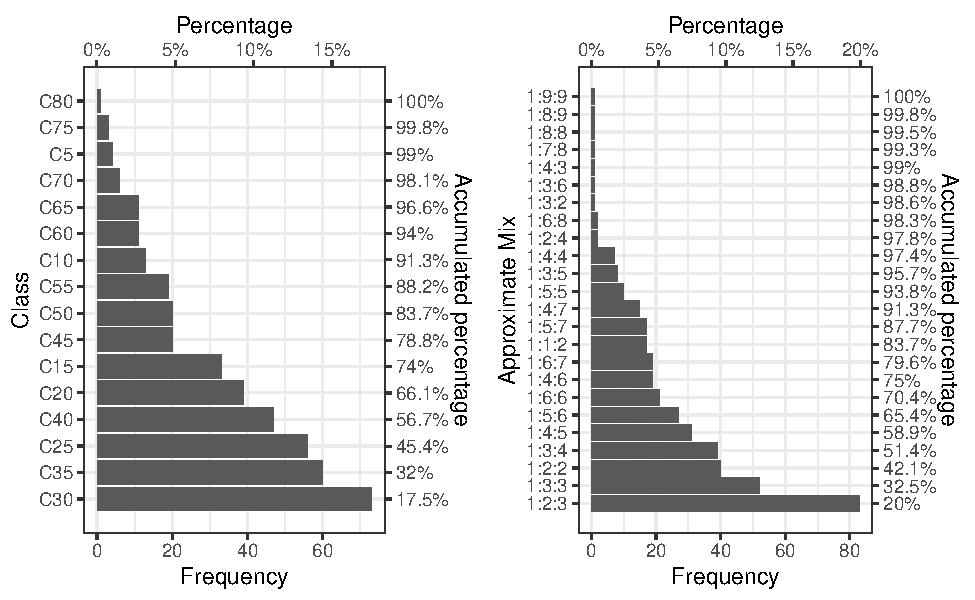
\includegraphics{CopyOfcapstone_files/figure-latex/stat-summ-categorical-1} 

}

\caption{Descriptive statistics - categorical variables}\label{fig:stat-summ-categorical}
\end{figure}

\hypertarget{correlation-between-ingredients-and-compressive-strength}{%
\subsubsection{Correlation between ingredients and compressive
strength}\label{correlation-between-ingredients-and-compressive-strength}}

The figure \ref{fig:correlation} shows the correlation of variables for
each set of ages (\ref{show-correlation}). The figure
\ref{fig:correlation-mpa} presents the same data, but instead of
correlating them all, it only correlates with the compressive strength,
showing the values in more detail (\ref{show-correlation-mpa}).

~

\begin{figure}

{\centering 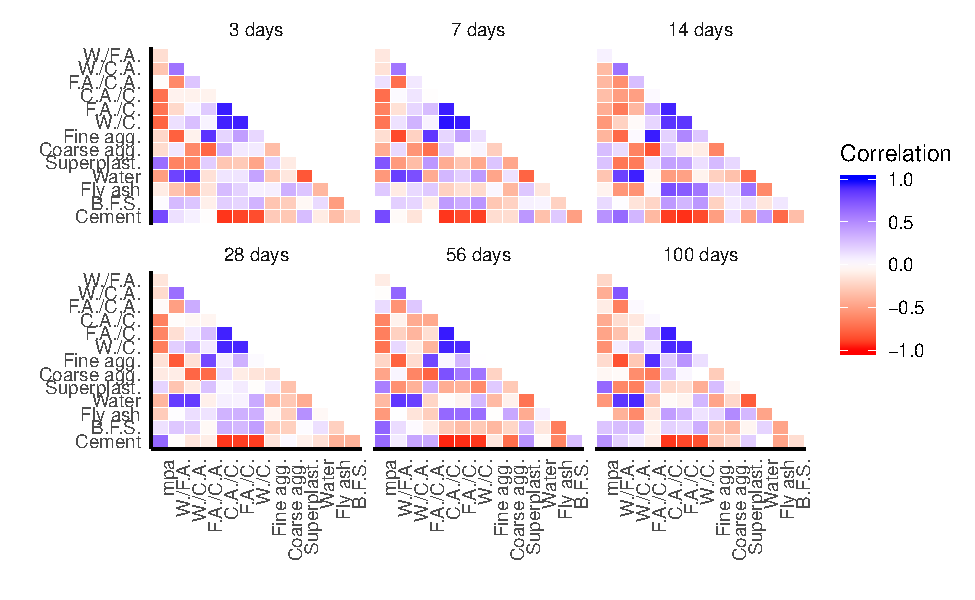
\includegraphics{CopyOfcapstone_files/figure-latex/correlation-1} 

}

\caption{Correlations at each age}\label{fig:correlation}
\end{figure}

\begin{figure}

{\centering 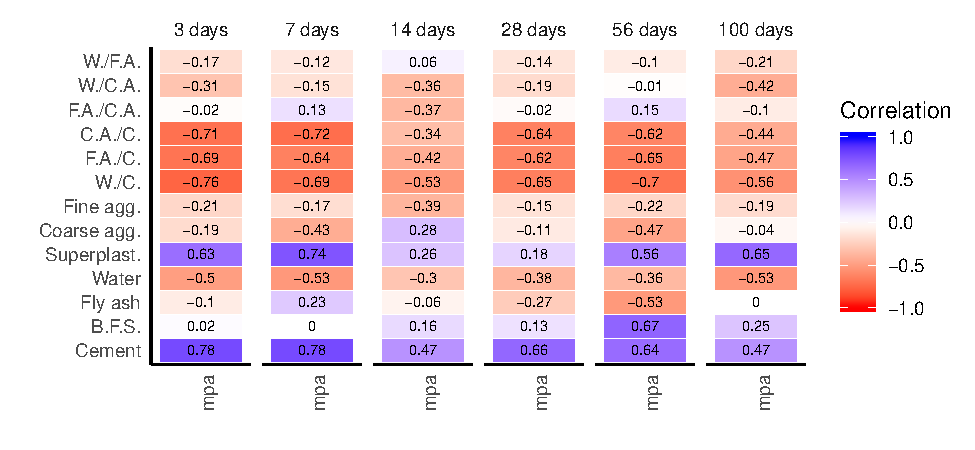
\includegraphics{CopyOfcapstone_files/figure-latex/correlation-mpa-1} 

}

\caption{Correlation of variables with compressive strength over time}\label{fig:correlation-mpa}
\end{figure}

The interpretation of the figure \ref{fig:correlation-mpa} suggests that
the strength of the concrete is positively related mainly to the cement
and superplasticizer ingredients and negatively to the water and fine
aggregate. The smaller the amount of cement for aggregates and water,
the more negatively they are correlated with compressive strength.

~

\begin{figure}

{\centering 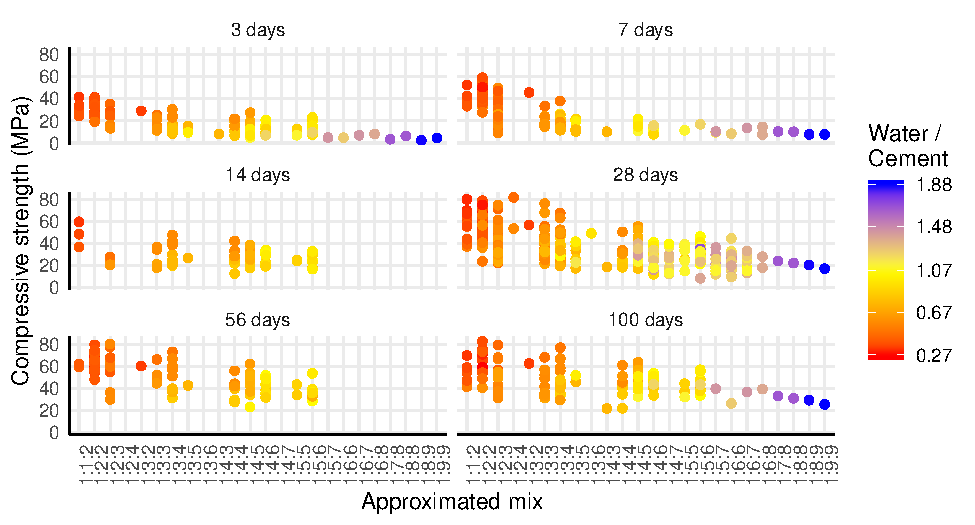
\includegraphics{CopyOfcapstone_files/figure-latex/mix-app-mpa-1} 

}

\caption{Relationship between approximated mix, water, MPa and age}\label{fig:mix-app-mpa}
\end{figure}

\begin{figure}

{\centering 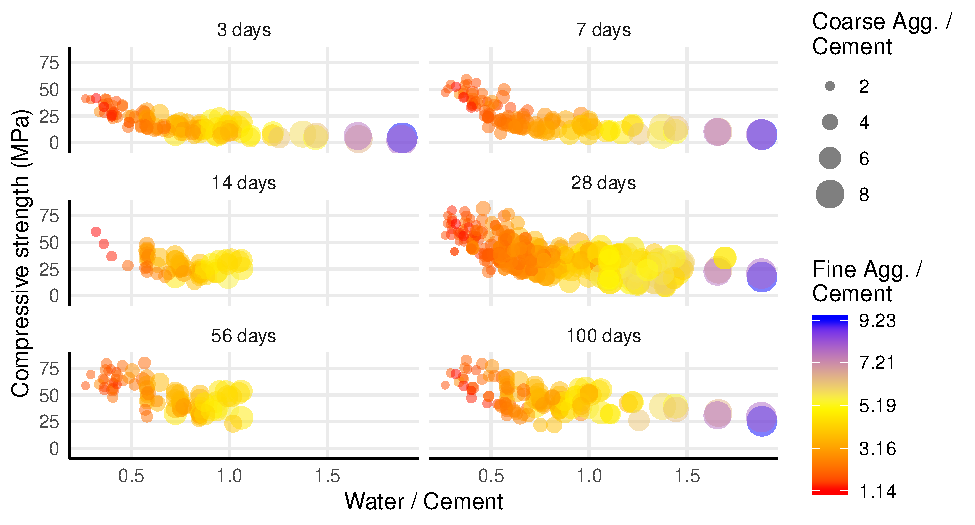
\includegraphics{CopyOfcapstone_files/figure-latex/mix-mpa-1} 

}

\caption{Relationship between concrete main features}\label{fig:mix-mpa}
\end{figure}

The figures \ref{fig:mix-app-mpa} and \ref{fig:mix-mpa} show the
relationship between the main ingredients (known as mix) in relation to
the compressive strength (\ref{show-mix-app-mpa} and
\ref{show-mix-mpa}). The interpretation of these figures shows that the
greater the amount of cement in relation to the other ingredients, the
greater the resistance to compression.

\hypertarget{variables-distribution}{%
\subsubsection{Variables distribution}\label{variables-distribution}}

The figure\ref{fig:vars-distribution} shows the distribution of
variables in the samples (\ref{show-vars-distribution}). It was
calculated using data only at 28 days.

~

\begin{figure}

{\centering 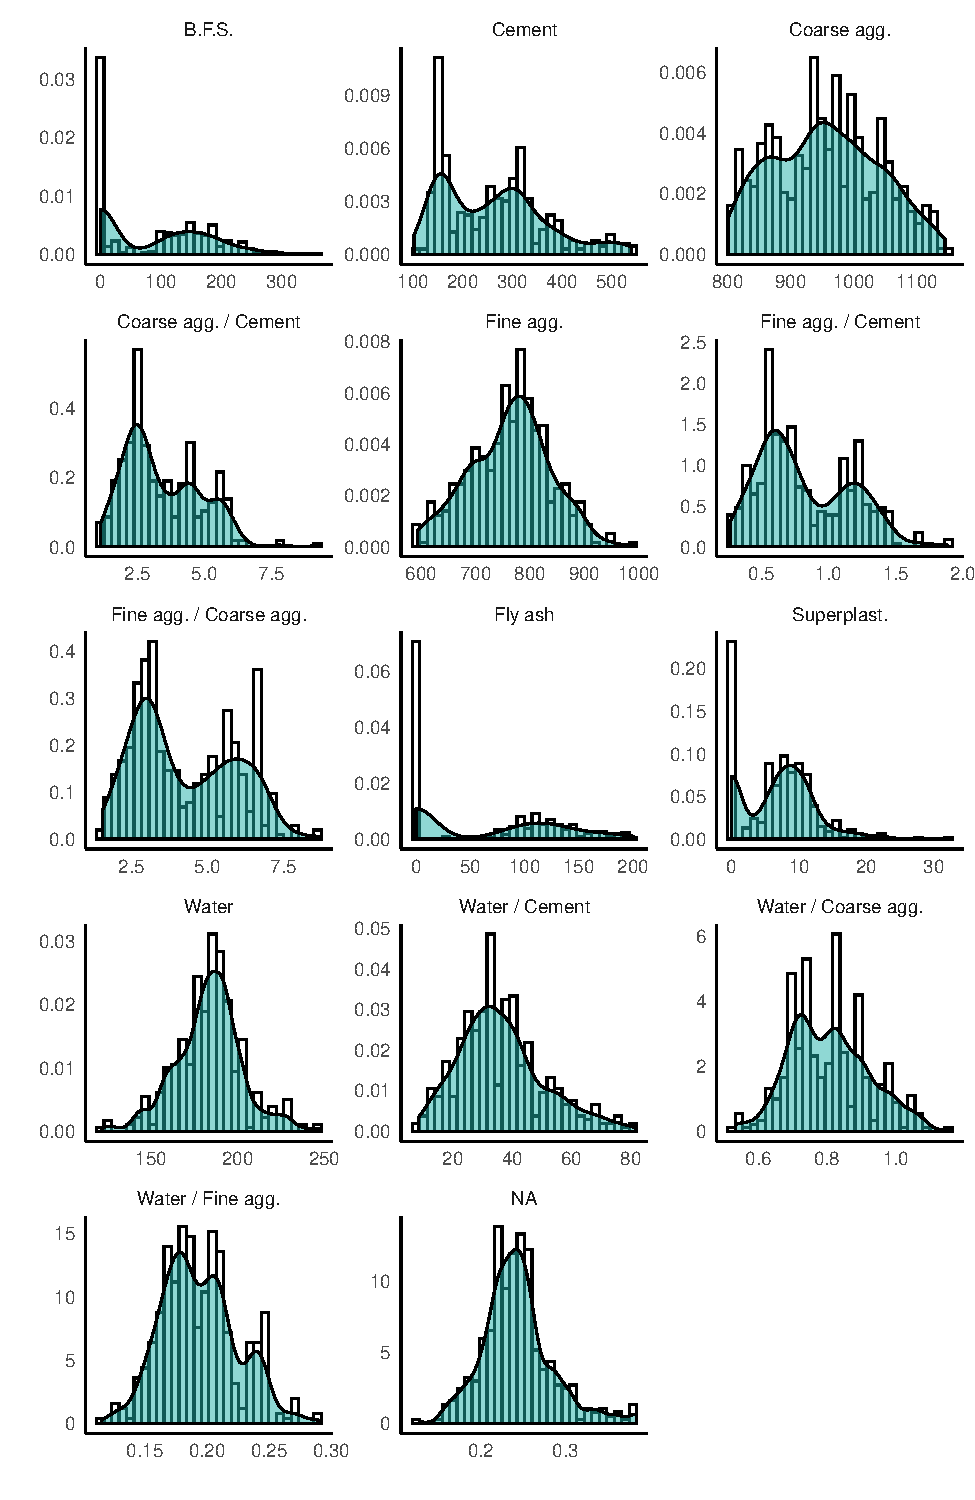
\includegraphics{CopyOfcapstone_files/figure-latex/vars-distribution-1} 

}

\caption{Variables distribution}\label{fig:vars-distribution}
\end{figure}

The figure \ref{fig:vars-distribution-time} shows the distribution of
ingredients and compressive strength for each set of ages
(\ref{show-vars-distribution-time}), in case of the 28 days it presents
the same information as the figure \ref{fig:vars-distribution}. It shows
that the resistance to compression gradually increases over time, as
expected. Furthermore it is seen that the concentration of the
ingredients can vary a lot when stratified by ages.

\begin{figure}

{\centering 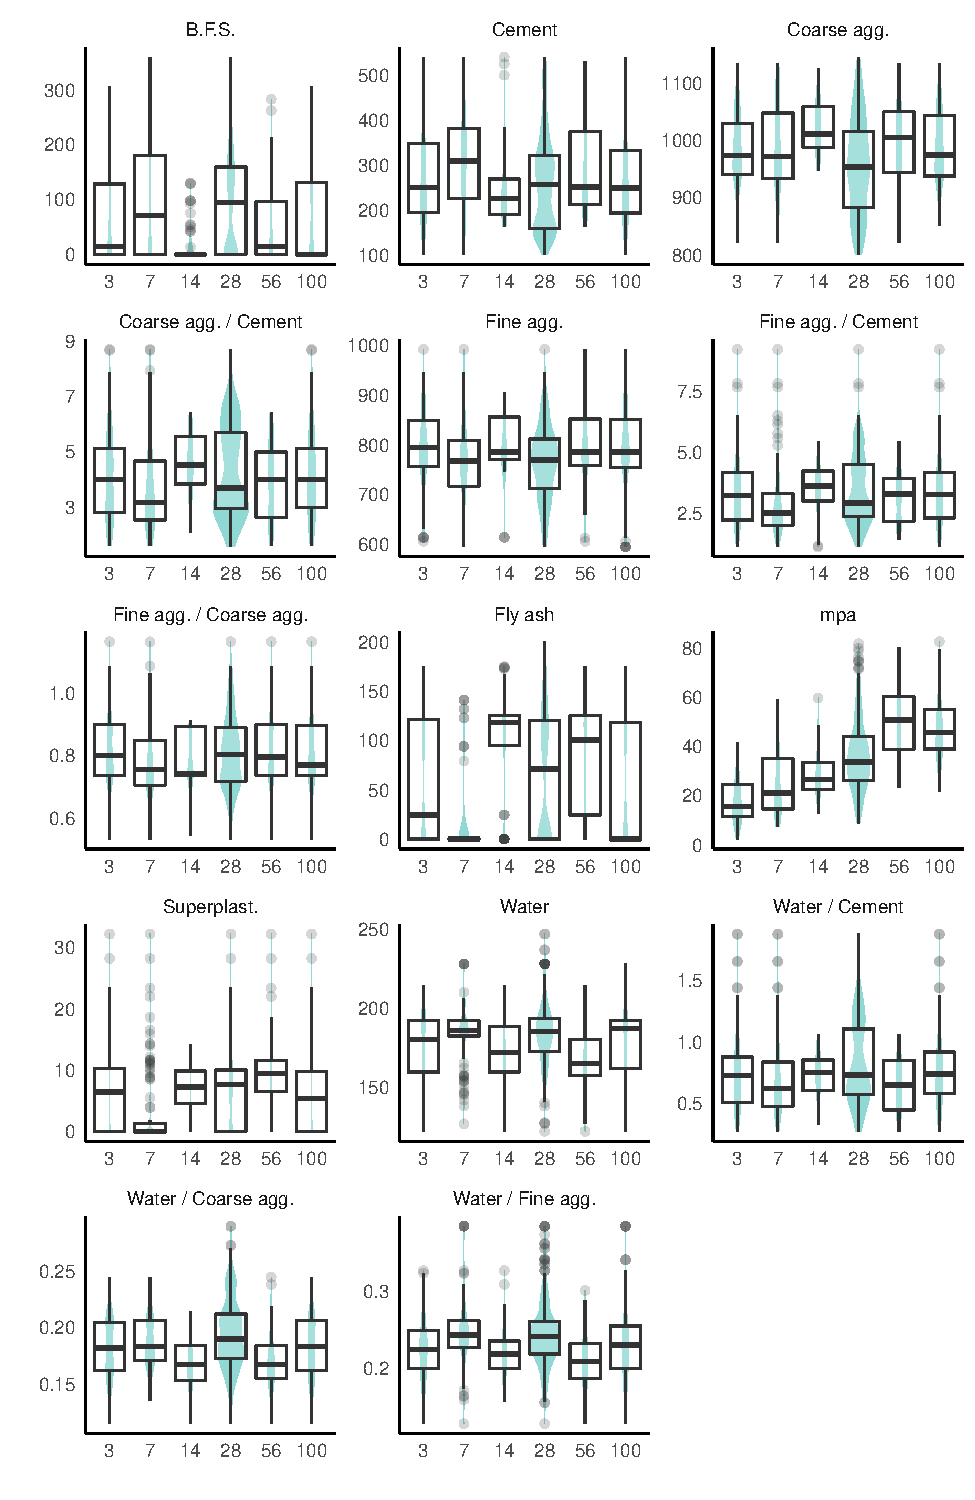
\includegraphics{CopyOfcapstone_files/figure-latex/vars-distribution-time-1} 

}

\caption{Variables distribution grouped by age}\label{fig:vars-distribution-time}
\end{figure}

\hypertarget{principal-component-analysis}{%
\subsubsection{Principal component
analysis}\label{principal-component-analysis}}

In the figure \ref{fig:pca}, using an alternative classification, the
principal component analysis was performed on the ingredients
(\ref{show-pca}). The classification separates concrete into 4 different
compressive strength groups, low up to \emph{20 MPa}, normal up to
\emph{40 MPa}, medium up to \emph{70 MPa} and high above that. It is
possible to notice that the groups overlap, but there is a
differentiation between the high and low group.

\begin{figure}

{\centering 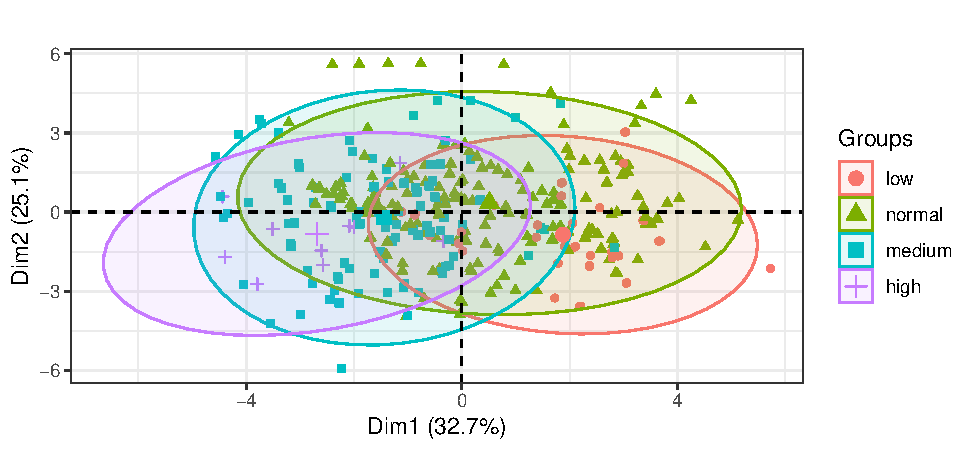
\includegraphics{CopyOfcapstone_files/figure-latex/pca-1} 

}

\caption{Principal component analysis on ingredients}\label{fig:pca}
\end{figure}

\hypertarget{literature-cited}{%
\section{Literature cited}\label{literature-cited}}

\hypertarget{refs}{}
\leavevmode\hypertarget{ref-Yeh1998}{}%
Yeh, I-Cheng. n.d. ``Modeling of Strength of High-Performance Concrete
Using Artificial Neural Networks.''
\url{https://doi.org/10.1016/S0008-8846(98)00165-3}.

\end{document}
